
\documentclass[border=15pt, multi, tikz]{standalone}
\usepackage{import}
\usepackage{xcolor}

% Define custom colors
\definecolor{ConvColor}{RGB}{255,213,79}      % Yellow for ConvNeXt
\definecolor{HexColor}{RGB}{129,199,132}       % Green for HexNeXt
\definecolor{TransColor}{RGB}{100,181,246}     % Blue for Transformer
\definecolor{HeadColor}{RGB}{240,98,146}       % Pink for Task Heads
\definecolor{InputColor}{RGB}{189,189,189}     % Gray for Input
\definecolor{TokenColor}{RGB}{186,104,200}     % Purple for Tokens

\usetikzlibrary{positioning, shapes, arrows.meta, calc, fit, backgrounds}

\begin{document}
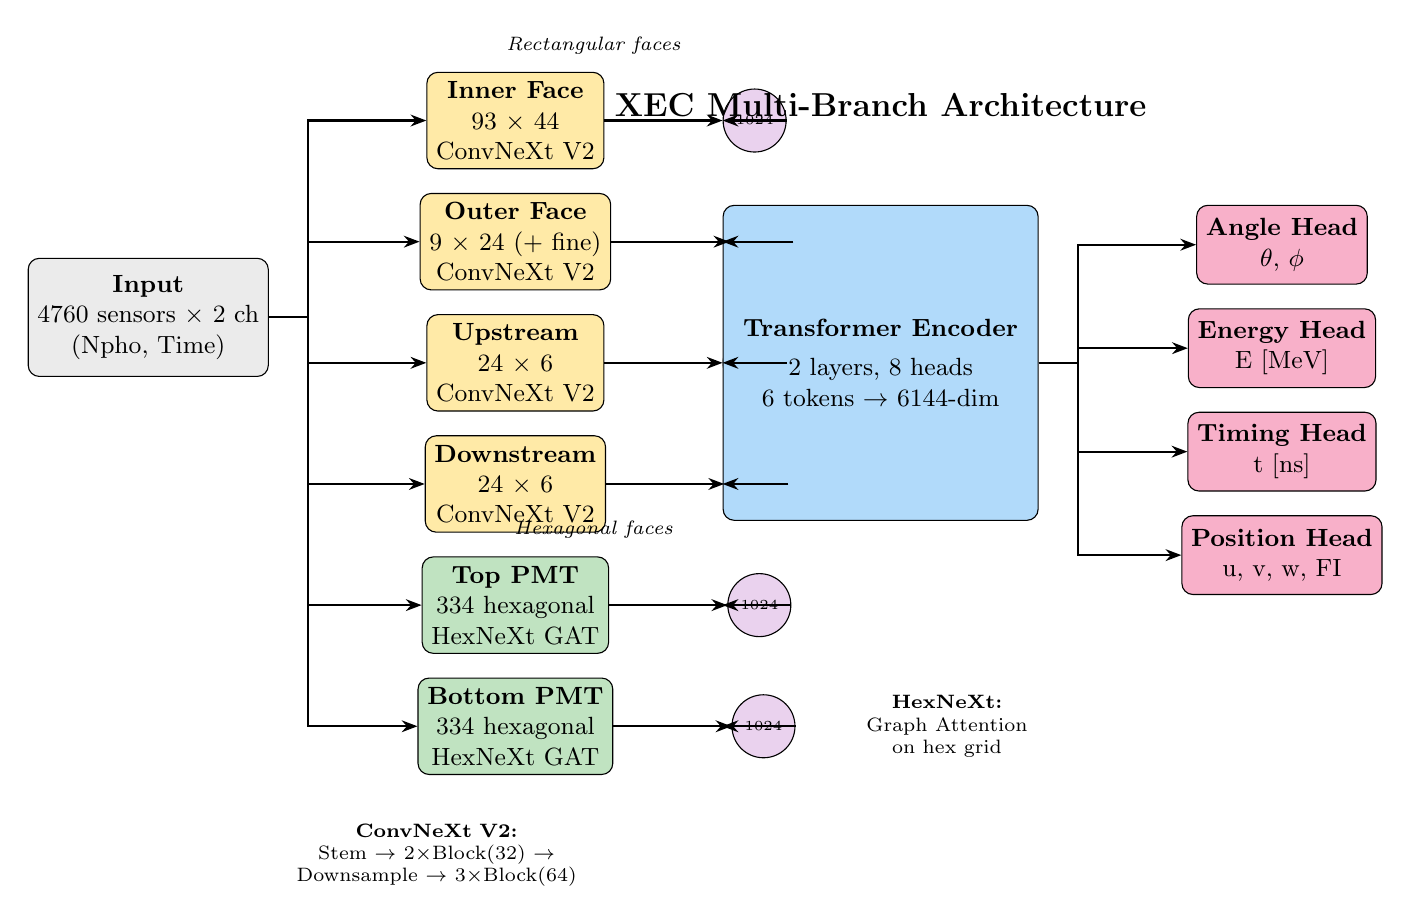
\begin{tikzpicture}[
    node distance=0.8cm,
    box/.style={rectangle, draw, rounded corners, minimum height=1cm, minimum width=2cm, align=center, font=\small},
    input/.style={box, fill=InputColor!30},
    conv/.style={box, fill=ConvColor!50},
    hex/.style={box, fill=HexColor!50},
    token/.style={circle, draw, fill=TokenColor!30, minimum size=0.8cm, font=\tiny},
    trans/.style={box, fill=TransColor!50, minimum width=4cm},
    head/.style={box, fill=HeadColor!50},
    arrow/.style={-{Stealth[length=2mm]}, thick},
    label/.style={font=\scriptsize, align=center},
]

% ============================================
% INPUT LAYER
% ============================================
\node[input, minimum width=3cm, minimum height=1.5cm] (input) {
    \textbf{Input}\\
    4760 sensors $\times$ 2 ch\\
    (Npho, Time)
};

% ============================================
% FACE ENCODERS - Rectangular (ConvNeXt)
% ============================================
\node[conv, right=2cm of input, yshift=2.5cm] (inner) {
    \textbf{Inner Face}\\
    93 $\times$ 44\\
    ConvNeXt V2
};

\node[conv, below=0.3cm of inner] (outer) {
    \textbf{Outer Face}\\
    9 $\times$ 24 (+ fine)\\
    ConvNeXt V2
};

\node[conv, below=0.3cm of outer] (us) {
    \textbf{Upstream}\\
    24 $\times$ 6\\
    ConvNeXt V2
};

\node[conv, below=0.3cm of us] (ds) {
    \textbf{Downstream}\\
    24 $\times$ 6\\
    ConvNeXt V2
};

% ============================================
% FACE ENCODERS - Hexagonal (HexNeXt)
% ============================================
\node[hex, below=0.3cm of ds] (top) {
    \textbf{Top PMT}\\
    334 hexagonal\\
    HexNeXt GAT
};

\node[hex, below=0.3cm of top] (bot) {
    \textbf{Bottom PMT}\\
    334 hexagonal\\
    HexNeXt GAT
};

% ============================================
% 1024-dim TOKENS
% ============================================
\node[token, right=1.5cm of inner] (t1) {1024};
\node[token, right=1.5cm of outer] (t2) {1024};
\node[token, right=1.5cm of us] (t3) {1024};
\node[token, right=1.5cm of ds] (t4) {1024};
\node[token, right=1.5cm of top] (t5) {1024};
\node[token, right=1.5cm of bot] (t6) {1024};

% ============================================
% TRANSFORMER FUSION
% ============================================
\node[trans, right=1.5cm of us, minimum height=4cm] (transformer) {
    \textbf{Transformer Encoder}\\[3pt]
    2 layers, 8 heads\\
    6 tokens $\rightarrow$ 6144-dim
};

% ============================================
% TASK HEADS
% ============================================
\node[head, right=2cm of transformer, yshift=1.5cm] (angle) {
    \textbf{Angle Head}\\
    $\theta$, $\phi$
};

\node[head, below=0.3cm of angle] (energy) {
    \textbf{Energy Head}\\
    E [MeV]
};

\node[head, below=0.3cm of energy] (timing) {
    \textbf{Timing Head}\\
    t [ns]
};

\node[head, below=0.3cm of timing] (position) {
    \textbf{Position Head}\\
    u, v, w, FI
};

% ============================================
% ARROWS - Input to Encoders
% ============================================
\draw[arrow] (input.east) -- ++(0.5,0) |- (inner.west);
\draw[arrow] (input.east) -- ++(0.5,0) |- (outer.west);
\draw[arrow] (input.east) -- ++(0.5,0) |- (us.west);
\draw[arrow] (input.east) -- ++(0.5,0) |- (ds.west);
\draw[arrow] (input.east) -- ++(0.5,0) |- (top.west);
\draw[arrow] (input.east) -- ++(0.5,0) |- (bot.west);

% ============================================
% ARROWS - Encoders to Tokens
% ============================================
\draw[arrow] (inner.east) -- (t1.west);
\draw[arrow] (outer.east) -- (t2.west);
\draw[arrow] (us.east) -- (t3.west);
\draw[arrow] (ds.east) -- (t4.west);
\draw[arrow] (top.east) -- (t5.west);
\draw[arrow] (bot.east) -- (t6.west);

% ============================================
% ARROWS - Tokens to Transformer
% ============================================
\draw[arrow] (t1.east) -- (t1.east -| transformer.west);
\draw[arrow] (t2.east) -- (t2.east -| transformer.west);
\draw[arrow] (t3.east) -- (t3.east -| transformer.west);
\draw[arrow] (t4.east) -- (t4.east -| transformer.west);
\draw[arrow] (t5.east) -- (t5.east -| transformer.west);
\draw[arrow] (t6.east) -- (t6.east -| transformer.west);

% ============================================
% ARROWS - Transformer to Heads
% ============================================
\draw[arrow] (transformer.east) -- ++(0.5,0) |- (angle.west);
\draw[arrow] (transformer.east) -- ++(0.5,0) |- (energy.west);
\draw[arrow] (transformer.east) -- ++(0.5,0) |- (timing.west);
\draw[arrow] (transformer.east) -- ++(0.5,0) |- (position.west);

% ============================================
% LABELS
% ============================================
\node[label, above=0.1cm of inner, xshift=1cm] {\textit{Rectangular faces}};
\node[label, above=0.1cm of top, xshift=1cm] {\textit{Hexagonal faces}};

% Architecture label
\node[font=\large\bfseries, above=1cm of transformer] {XEC Multi-Branch Architecture};

% Encoder details (optional)
\node[label, below=0.5cm of bot, xshift=-1cm, text width=4cm] {
    \textbf{ConvNeXt V2:}\\
    Stem $\rightarrow$ 2$\times$Block(32) $\rightarrow$\\
    Downsample $\rightarrow$ 3$\times$Block(64)
};

\node[label, right=0.3cm of t6, text width=3cm] {
    \textbf{HexNeXt:}\\
    Graph Attention\\
    on hex grid
};

\end{tikzpicture}
\end{document}
